\section{Results}
\label{sec:results}

\subsection{Speckle Motion Detection}

The results confirmed that the motion of speckle patterns was successfully detected using the discrete photodiode array. 
Phase-shifted signals were observed across multiple photodiodes, indicating the presence of a moving speckle pattern. 
This phase information confirmed that the photodiode array could effectively visualize the dynamic speckle motion. 
The use of an IR LED further validated that the detected signals originated from laser speckle patterns and not from external light interference.

\subsection{Signal-to-Noise Ratio (SNR) Analysis}

The SNR analysis demonstrated a positive correlation between the number of active lasers in the square array and the measurement quality. 
Incremental activation of the lasers resulted in an improvement in SNR, as shown in Figure~\ref{fig:laser_snr}. 
The power spectral density analysis highlighted the 133 Hz vibration component of the piezo disc, with an R² value of 0.60 indicating a moderately strong relationship between the number of lasers and SNR enhancement.

Control experiments with all lasers turned off verified that the observed signals originated from the laser speckle patterns and not from other sources. 
These results support the hypothesis that the use of multiple lasers enhances the SNR, improving the sensitivity of the system.

\subsection{Circuit Performance}

The custom-designed PCB and amplifier circuit were validated using SPICE simulations and experimental measurements. 
The Bode plot in Figure~\ref{fig:bodeplot} demonstrated a stable frequency response with high gain, while the transient response shown in Figure~\ref{fig:transient} confirmed system stability. 
Noise measurements (Figure~\ref{fig:totalnoise}) indicated a low total noise level, making the circuit suitable for laser speckle detection.

\subsection{Impact of Experimental Parameters}

The experiments revealed several critical factors impacting the measurement results. 
The PCB required thorough cleaning with IPA and compressed air to eliminate flux residue, as any remaining contaminants introduced noise. 
Additionally, conducting experiments in a light-controlled environment was essential to prevent saturation of the opamp and ensure reliable data capture. 
Dot projector alignment, facilitated by cameras, is critical for ensuring consistent speckle patterns and uniform distribution across the photodiode array.

\subsection{Limitations}
The opamp saturated in sunlight, rendering the signal irrecoverable in such conditions. Dot projectors cannot be effectively used as the reflected light is too weak.
Furthermore, the bandwidth of the system is limited to 1kHz.


\begin{figure*}[t]
    \centering
    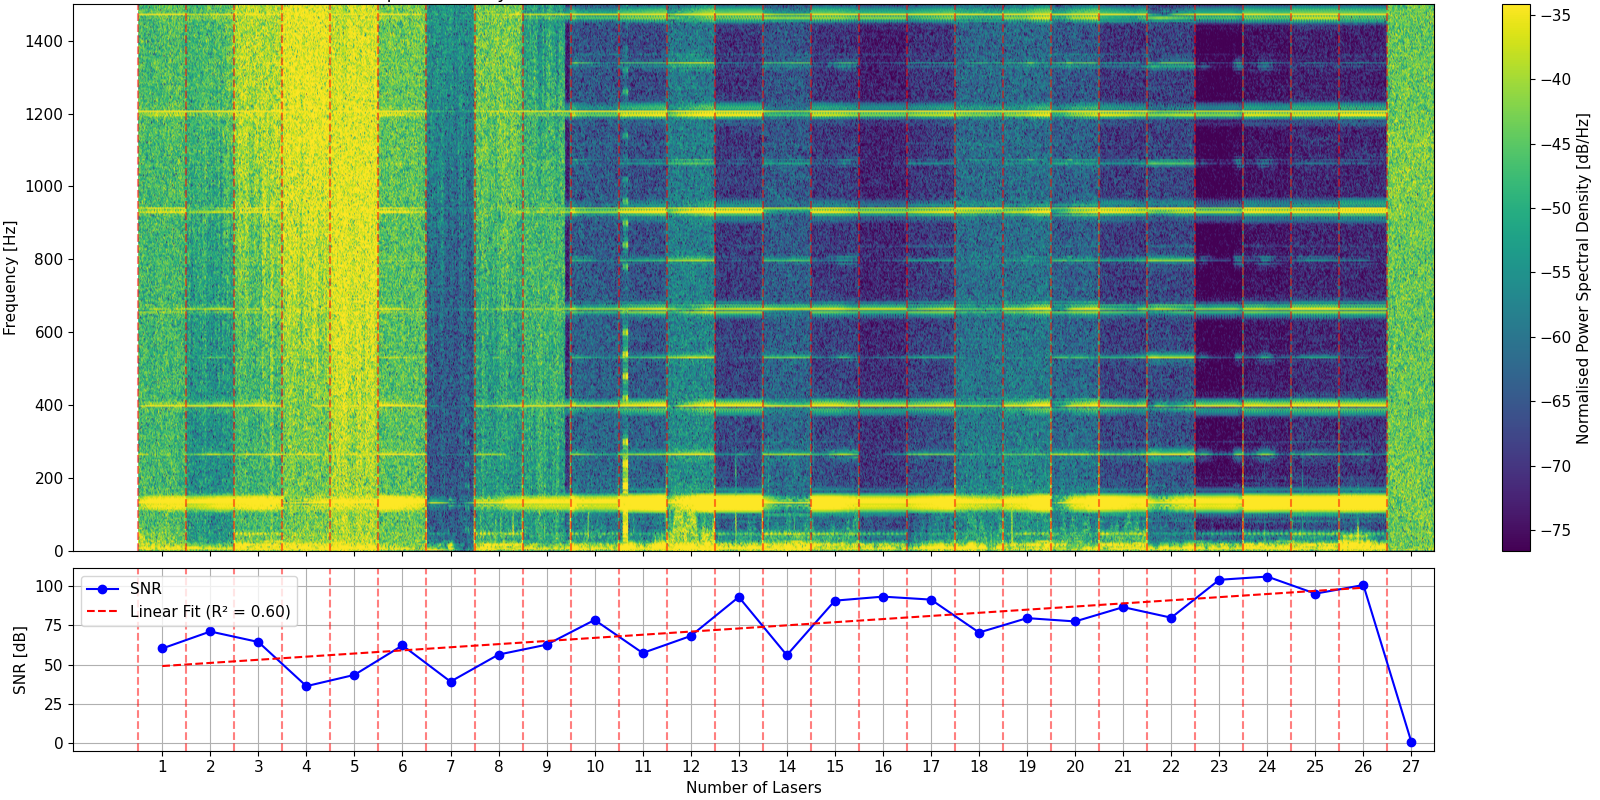
\includegraphics[width=\textwidth]{figures/results/multilaser_spectrogram}
    \caption{Spectral analysis of a 133~Hz surface vibration under different laser configurations. 
    Top: Power spectral density showing the target frequency component. Bottom: SNR improvement with increasing number of active lasers.}
    \label{fig:laser_snr}
\end{figure*}